%!TEX root = ../mtrgrmetod.tex
\chapter{Розрахунок модуля оперативного запам'ятовувального пристрою}

%При матричной организации ИМС памяти (рис. 5.6) реализуется координатный принцип адресации ячеек. Адрес ячейки, поступающий по шине адреса ВМ, пропускается через логику выбора, где он разделяется на две составляющие: адрес строки и адрес столбца. Адреса строки и столбца запоминаются соответственно в регистре адреса строки и регистре адреса столбца микросхемы. Регистры соединены каждый со своим дешифратором. Выходы дешифраторов образуют систему горизонтальных и вертикальных линий, к которым подсоединены запоминающие матрицы, при этом каждый ЗЭ расположен на пересечении одной горизонтальной и одной вертикальной линии. 

%\section{ttt}

Незалежно від того, яким чином організована мікропроцесорна система, в її складі в будь-якому випадку має бути запам'ятовувальний пристрій. Як правило, в складі такої системи можна побачити постійний запам'я\-то\-ву\-валь\-ний пристрій та оперативний запам'ятовувальний пристрій, які поділять між собою адресний простір мікропроцесора, але, в окремих випадках номенклатура пристроїв зберігання інформації в складі мікропроцесорної системи буде ширшою.

%\vspace{8mm}

\section{Класифікація запам'ятовувальних пристроїв}

Класифікувати запам'ятовувальні пристрої (ЗП), які використовуються в мікропроцесорних системах сьогодні, можна за такими ознаками:
\begin{enumerate}
 \item \textbf{за місцем} розташування відносно обчислювального прис\-трою:
   \begin{enumerate}
   \item зовнішні ЗП,
   \item внутрішні ЗП;
   \end{enumerate}
 \item \textbf{за призначенням}:
   \begin{enumerate}
   \item надоперативні ЗП (НОЗП) -- мають швидкодію, сумірну зі швидкодією обчислювального пристрою. Використо\-ву\-ють\-ся для зберігання результатів проміжних операцій. У мікропроцесорах роль НОЗП виконує регістрова пам'ять -- вбудовані в мікропроцесор регістри загального призначення;
   \item оперативні ЗП (ОЗП) -- енергозалежні ЗП, вико\-рис\-то\-ву\-ють\-ся для первинного зберігання інформації, що вво\-дить\-ся. При відсутності живлення інформація втрачається;
   \item постійні ЗП (ПЗП) -- енергонезалежні ЗП, ви\-ко\-рис\-то\-ву\-ють\-ся для зберігання інформації і за відсутності напруги живлення;
   \item буферні ЗП (БЗП) -- призначені для проміжного зберігання інформації при її обміні між пристроями, що працюють з різною швидкістю. Цю роль виконують регістрові схеми або ОЗП малого обсягу;
   \item зовнішні ЗП (ЗЗП) використовуються для зберігання великого обсягу інформації на зовнішньому, щодо обчислювального пристрою, носії, як правило, магнітному;
   \end{enumerate}\newpage
 \item \textbf{за фізичним принципом} дії:
   \begin{enumerate}
   \item магнітні,
   \item напівпровідникові,
   \item оптичні;
   \end{enumerate}
 \item \textbf{за способом зберігання} інформації:
   \begin{enumerate}
   \item статичні,
   \item динамічні;
   \end{enumerate}
 \item \textbf{за способом доступу} до комірок:
   \begin{enumerate}
   \item адресні ЗП -- код на адресному вході вказує на комірку, з якою ведеться обмін даними;
   \item послідовні ЗП -- звернення до комірки з заданою адресою передбачає виконання попередніх звернень до всіх комірок, які мають молодші адреси;
   \item асоціативні ЗП -- пошук інформації відбувається за деякою ознакою, а не за її розташуванням в пам'яті.
   \end{enumerate}        
\end{enumerate}

\vspace{0.1cm}

Для позначення запам'ятовувальних пристроїв ОЗП та ПЗП з одної класифікаційної категорії «за призначенням» в літературі використовують сталі англомовні скорочення RAM та ROM. Однак ці абревіатури характеризують пристрої з різних сторін. Так, RAM (\textit{англ. Random Access Memory -- пам'ять з довільним доступом}) вказує на те, що для доступу до певної комірки не потрібно попередньо звертатись до комірок з молодшими адресами. Сама ж пам'ять при цьому може бути енергозалежною або енергонезалежною. Так само ROM (\textit{англ. Read Only Memory -- пам'ять тільки для читання}) свідчить про те, що в такий пристрій записувати не можна. Але енергонезалежність пристрою передбачає і можливість запису. Не зважаючи на таку неточність ці абревіатури залишаються сталими та широковживаними у сфері комп'ютерної техніки для позначення ОЗП та ПЗП.

В свою чергу оперативні запам'ятовувальні пристрої RAM по\-ді\-ля\-ють\-ся на статичні -- SRAM (\textit{англ. Static RAM}) та динамічні -- DRAM (\textit{англ. Dynamic RAM}).

У статичних ОЗП запам'ятовувальними елементами є тригери, на відміну від динамічних ОЗП, в яких дані зберігають у вигляді зарядів конденсаторів, що утворюються елементами МОН-структур. Особливістю динамічних ОЗП є те, що запам'ятовувальні конденсатори з часом розряджаються, тому періодично дані мають регенеруватися.

Щільність пакування динамічних елементів пам'яті в кілька разів вища, ніж статичних, тому динамічні ОЗП характеризуються найбільшою інформаційною ємністю і невисокою вартістю, але мають більше енергоспоживання і меншу швидкодію.

\newpage

Постійна пам'ять типу ROM має такі різновиди:
\begin{enumerate}
\item інтегральні схеми, які програмуються при виготовленні з допомогою масок -- ``маскові'' ПЗП або ROM(M);
\item пам'ять, що програмується користувачем, -- ППЗП (програмовані ПЗП):
  {\begin{itemize}
  \item PROM -- дані в пам'ять записуються один раз,
  \item EPROM та EEPROM -- вміст пам'яті може бути змінений шляхом видалення інформації та запису нової.  
  \end{itemize}}
\end{enumerate}

В EPROM видалення інформації відбувається шляхом опромінення кристала ультрафіолетовими променями (ППЗП-УФ -- ПЗП з можливістю перепрограмування шляхом видалення інформації УФ опроміненням). В EEPROM видалення інформації відбувається електричними сигналами (ППЗП-ЕС -- ПЗП з можливістю перепрограмування з використанням електричних сигналів). Запис даних в обох випадках (EPROM та EEPROM) відбувається з використанням електричних сигналів.

%----------------------------------------------------------------
\section{Способи збільшення інформаційного обсягу ЗП}

При проектуванні модуля ЗП на заданих великих інтегральних схемах  (ВІС) часто доводиться вирішувати задачу збільшення загальної інформаційної ємності пам'яті мікропроцесорної системи. Як правило, ця задача вирішується трьома способами: 

\begin{enumerate}
 \item{збільшенням розрядності даних (розрядності слів),}
 \item{збільшенням кількості слів, що адресуються (збільшення роз\-ряд\-нос\-ті шини адреси),}
 \item{комбінований.}
\end{enumerate}

\begin{center}
\textit{Збільшення розрядності даних}
\end{center}

Збільшення розрядності даних досягається шляхом паралельного з'єднання адресних ліній декількох мікросхем ЗП. В такому випадку на всі мікросхеми ЗП одночасно подається однакова адреса. Входи $\overline{CS}$ та \textit{$\overline{W}\!\!$/$R$} з'єднуються між собою також паралельно, що забезпечує подачу сигналів керування на всі мікросхеми одночасно. Таким чином в довільний момент часу для обміну даними доступні всі мікросхеми ЗП.

В наведеному прикладі (рис.~\ref{fig:sch1}) ємність одної інтегральної схеми буде визначатись як 

$$M1 = 2^{10}\cdot1 = 1024~\text{(біти)},$$

\noindent
а ємність всієї структури

$$M = M1\cdot8 = 2^{10}\cdot1\cdot8 = 8192~\text{(біти)} = 1~\text{(Кбайт)}.$$

\begin{figure}[h]
%\noindent
\centering
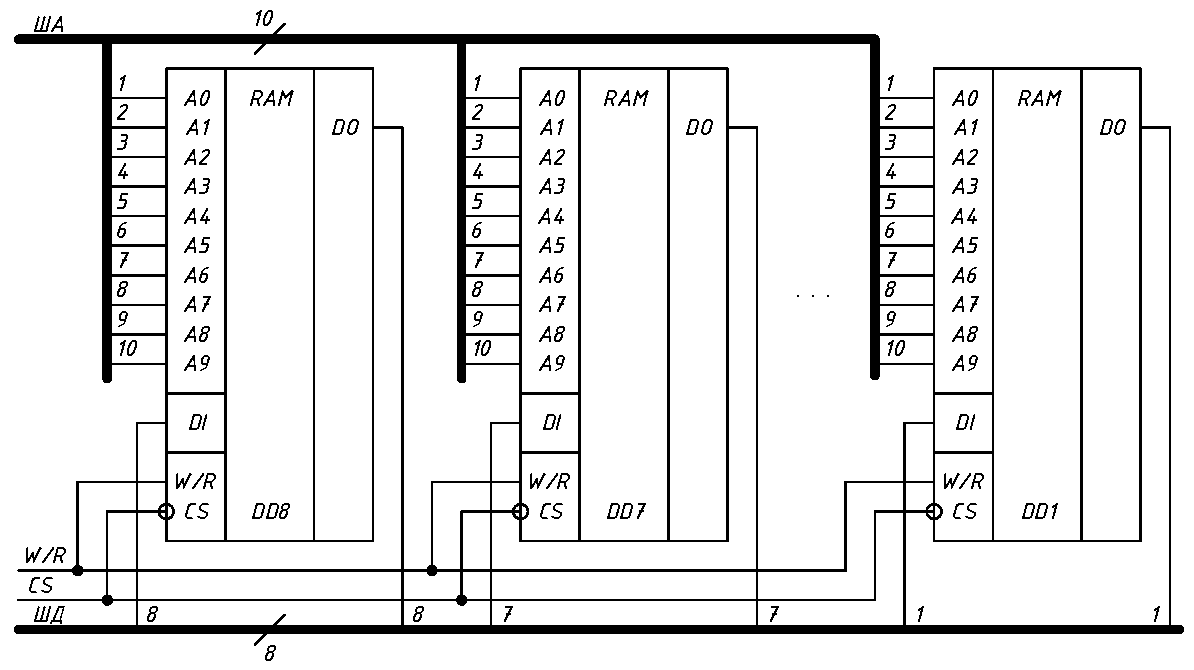
\includegraphics[width=\textwidth]{img/sch1-crop.pdf}
\caption{Збільшення розрядності даних}
\label{fig:sch1}
\end{figure}

Загальна інформаційна ємність в такому випадку змінюється за рахунок збільшення розрядності слів, що адресуються (з 1 біта для окремої ВІС до 1 байта для всього модуля ОЗП). Розрядність адреси ж всього модуля ОЗП залишається незмінною і збігається з розрядністю окремої ВІС, що дозволяє адресувати $2^{10} = 1024$ слова.  

\begin{center}
\textit{Збільшення кількості слів}
\end{center}

Для збільшення кількості слів, що адресуються, ви\-ко\-рис\-то\-ву\-єть\-ся дешифратор (\textit{англ. Decoder -- дешифратор}), на входи якого по\-да\-ють\-ся старші розряди шини адреси. Входи $\overline{CS}$ мікросхем ЗП під'єд\-ну\-ють\-ся до відповідних виходів дешифратора. Вхід $E$ дешифратора використовується як вхід дозволу роботи всієї схеми та використовується зовнішніми пристроями як вхід вибору кристала $\overline{CS}$. Проте в довільний момент часу для обміну даними доступна лише одна мікросхема ЗП в модулі. Входи \textit{$\overline{W}\!\!$/$R$} ЗП з'єднуються паралельно.

В наведеному прикладі (рис.~\ref{fig:sch2}) розрядність шини адреси збільшується з використанням дешифратора \textit{DD5}, на входи якого подаються старші розряди шини адреси. Входи $\overline{CS}$ окремих ВІС під'єднуються до відповідних виходів дешифратора. Вхід $E$ дешифратора використовується як вхід дозволу роботи всієї схеми та ідентифікується зовнішніми пристроями як вхід вибору кристала $\overline{CS}$. Входи \textit{$\overline{W}\!\!$/$R$} окремих ВІС з'єднуються між собою.

\begin{figure}[h]
%\noindent
\centering
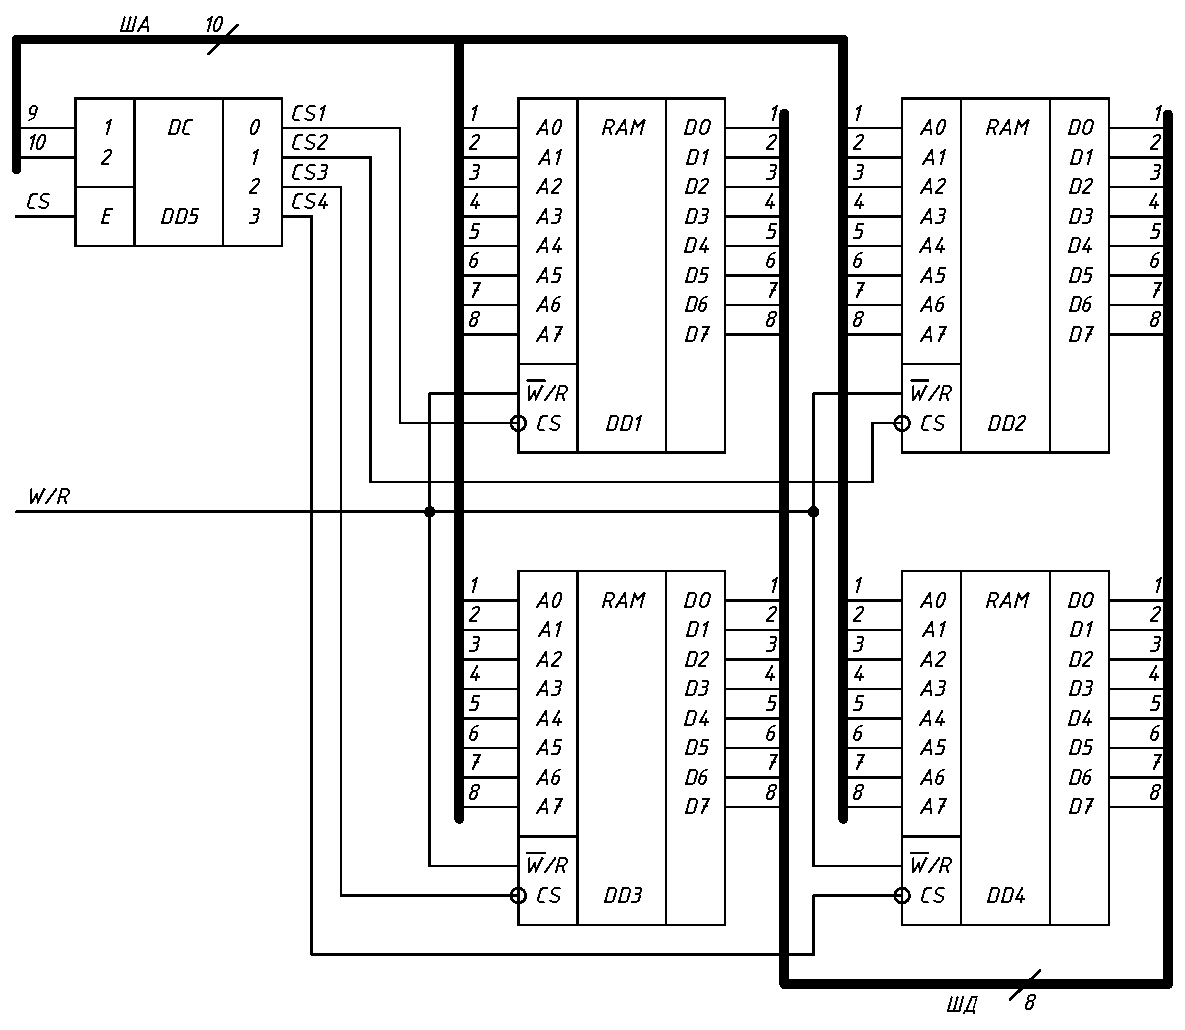
\includegraphics[width=\textwidth]{img/sch2(2)-crop.pdf}
\caption{Збільшення розрядності шини адреси}
\label{fig:sch2}
\end{figure}

Інформаційна ємність одної інтегральної схеми буде визначатись як

$$M1 = 2^{8}\cdot8 = 2048~\text{(бітів)},$$    

\noindent
а ємність всієї структури 

$$M = M1\cdot4 = 2^{8}\cdot8\cdot4 = 8192~\text{(біти)} = 1~\text{(Кбайт)}.$$

Загальна інформаційна ємність в такому випадку змінюється за рахунок збільшення кількості слів, що адресуються (з 256 для окремої ВІС до 1024 для всього модуля ОЗП). Розрядність слова залишається сталою як для модуля ОЗП в цілому, так і для окремої ВІС і складає 8~бітів. 

\begin{center}
\textit{Комбінований}
\end{center}

Комбінований спосіб передбачає і збільшення розрядності даних, і збільшення кількості слів, що адресуються. В такому випадку модуль ОЗП буде складатись із блоків, підключених за схемою збільшення розрядності шини адреси, а блоки збираються за схемою збільшення роз\-ряд\-нос\-ті даних.  

В наведеному прикладі (рис.~\ref{fig:sch3}) модуль ОЗП складається з чотирьох блоків організованих як $256\times8$, забезпечуючи загальну ємність запам'ятовувального пристрою 1024 байти або 1 Кбайт. В свою чергу кожен окремий блок складається з восьми ВІС, організованих як $256\times1$, здатних зберігати 256 бітів інформації.  

\begin{figure}[h]
%\noindent
\centering
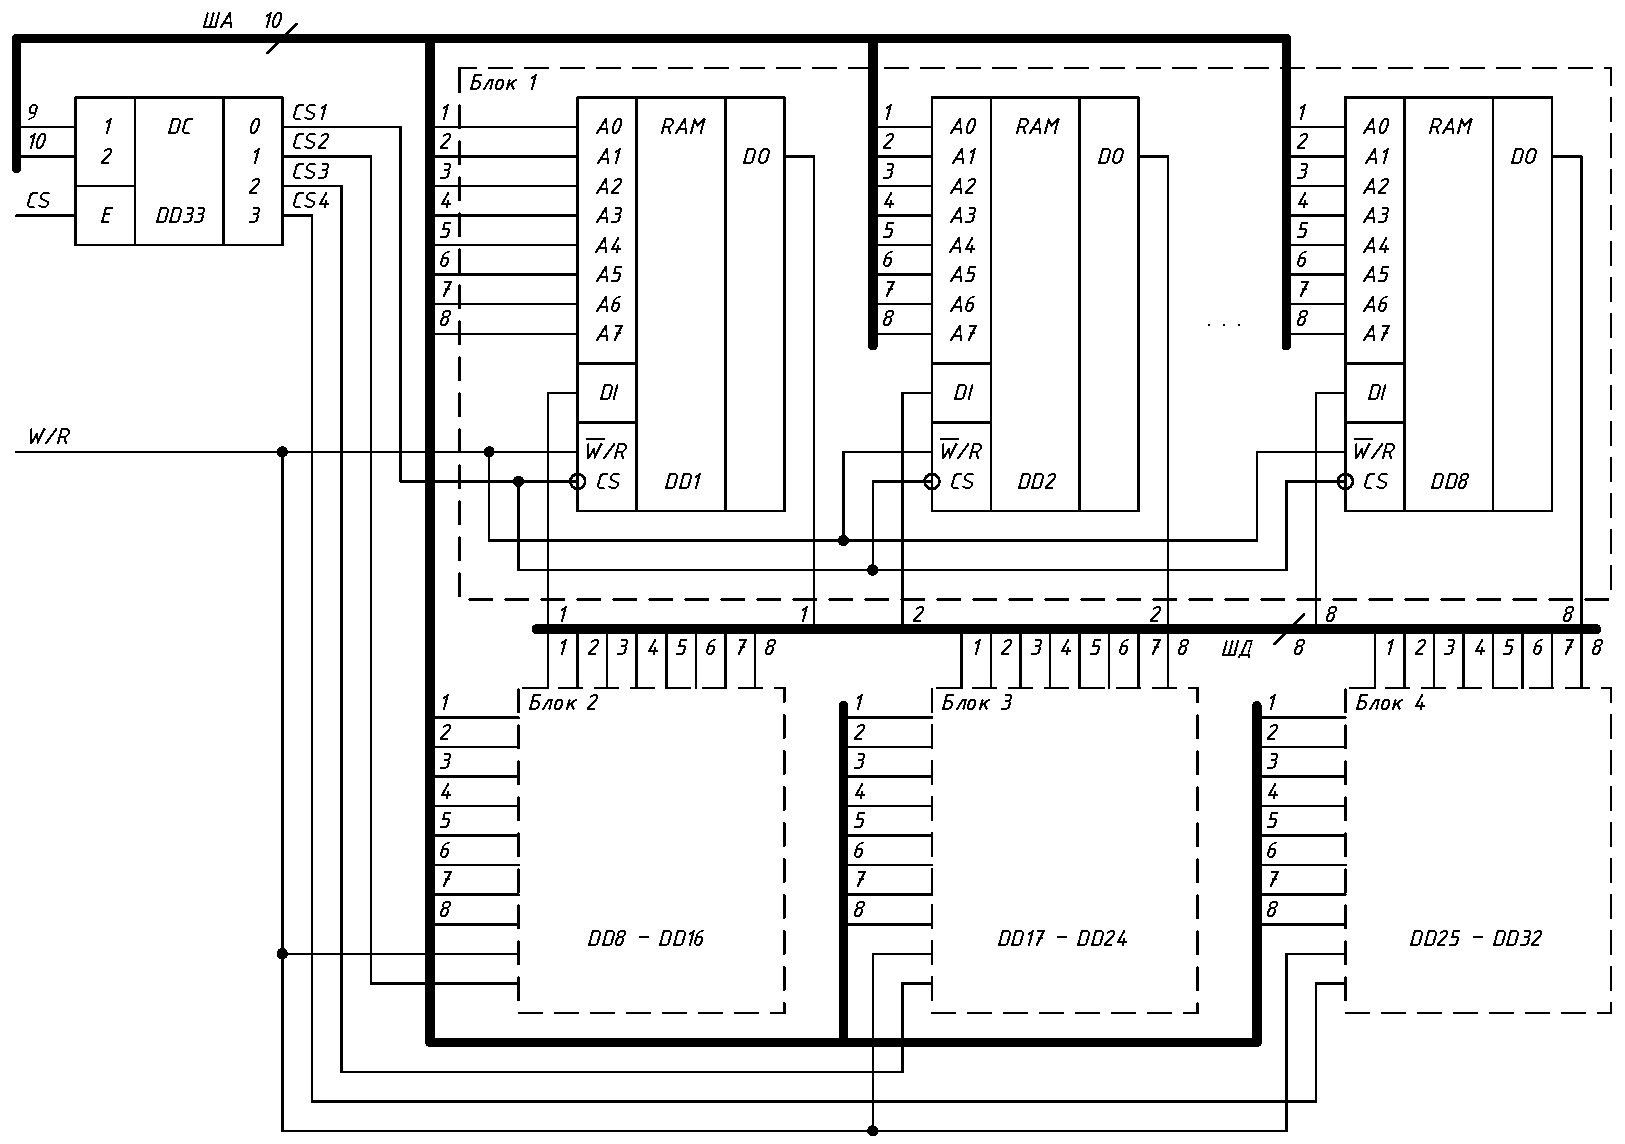
\includegraphics[width=0.99\textwidth]{img/sch3-crop.pdf}
\caption{Комбінований метод}
\label{fig:sch3}
\end{figure}

Інформаційна ємність одної інтегральної схеми буде визначатись як

$$M1 = 2^{8}\cdot1 = 256~\text{(бітів)}.$$    

В свою чергу інформаційна ємність блока буде визначатись як добуток інформаційної ємності одної ВІС на їх кількість в блоці

$$M_{\text{Б}} = 2^{8}\cdot1\cdot8 = 2048~\text{(біта)} = 256~\text{(байтів)},$$ 

\noindent
а інформаційна ємність всієї структури становитиме 

$$M = M_{\text{Б}}\cdot4 = 2048\cdot4 = 8192~\text{(біти)} = 1~\text{(Кбайт)}.$$

Загальна iнформацiйна ємнiсть в такому випадку змiнюється як за рахунок збiльшення розрядностi слiв, що адресуються (з 1 бiта для окремої ВIС до 1 байта для окремого блока), так і за рахунок збільшення кількості слів, що адресуються (з 256 слів для окремої ВІС або окремого блока до 1024 для всього модуля ОЗП). 

Наведені приклади наочно демонструють рiзнi підходи до вирішення задачі збільшення інформаційної ємності ЗП до 1 Кбайта. Очевидно, що в кожному окремому випадку саме заданий тип ВІС буде визначати спосіб проектування ОЗП.

\section{Розрахунок модуля ОЗП}

Базові розрахунки направлені на визначення кількості ВІС, потрібних для отримання шуканої інформаційної ємності всього модуля, та типу дешифратора для забезпечення коректного дешифрування адреси. Розглянемо на прикладі:

%---------------------------------------------------------------
%                         завдання
\par\bigskip 
\noindent\centerline{\begin{minipage}{0.95\textwidth}
\textit{розрахувати модуль ОЗП 64$\times$8 на основі мікросхем пам’яті 16$\times$4 із Z-станом. 	Накреслити схему електричну принципову модуля ОЗП для підключення до мікропроцесора. Для керування модулем використати лінії $\overline{CS}$ та          $\overline{W}\!\!$/$R$.}
\end{minipage}}\par\bigskip

1.~Визначаємо шукану інформаційну ємність модуля ОЗП в бітах

$$M = 64\cdot8 = 512~\text{(бітів)}.$$

2.~Визначаємо кількість мікросхем, що потрібні для реалізації необхідної розрядності даних (паралельне з'єднання ВІС). Розрядність заданої ВІС -- 4, розрядність даних, що вимагається завданням, -- 8, отже потрібно паралельно з'єднати дві мікросхеми.

Інформаційна ємність одної мікросхеми становитиме

$$M1 = 16\cdot4 = 64~\text{(біти)}.$$

Інформаційна ємність двох мікросхем, поєднаних в блок для розширення розрядності, становитиме

$$M_{\text{Б}} = M1\cdot2 = 16\cdot4\cdot2 = 128~\text{(бітів)}.$$

Розширення розрядності не забезпечує потрібної інформаційної ємності ОЗП, відповідно, доведеться використати комбінований спосіб збільшення обсягу ЗП.

\vspace{5mm}

3.~Визначаємо кількість блоків $k$, потрібних для реалізації шуканого обсягу $M$

$$k = \frac{M}{M_{\text{Б}}} = \frac{512}{128} = 4~\text{(блоки)}.$$

Блоки будемо підключати за схемою розширення розрядності шини адреси, тому потрібно буде використати дешифратор на чотири виходи (два входи).

Шина адреси модуля ОЗП шуканої інформаційної ємності шестирозрядна ($64 = 2^{6}$). Старші два розряди заводяться на входи дешифратора, молодші розряди, що залишились, заводяться паралельно на кожну окрему ВІС. Виходи дешифратора з'єднуються з входами вибору окремих блоків (\textit{CS1 -- CS4}), а лінія керування \textit{$\overline{W}\!\!$/$R$} підключається до відповідного входу кожної окремої ВІС в модулі (додаток \ref{apdx:ozpsch}).


